\documentclass{article}

\usepackage{url} 
\usepackage{geometry,afterpage}
\usepackage{pdfpages}
\usepackage{lastpage}
\usepackage{fancyhdr}
\usepackage{ngerman}
\usepackage{listings}

\usepackage{floatrow}
\usepackage[tableposition=top]{caption}
\floatsetup[table]{capposition=top}

\usepackage{amsmath, amssymb}

\usepackage[utf8]{inputenc}


\usepackage[numbib]{tocbibind}



\newcommand\twodigits[1]{%
   \ifnum#1<10 0#1\else #1\fi
}



\lhead{Hall Effekt}
\rhead{07.05.2021\\ J. Winkler}
%\cfoot{\twodigits{\thepage}~/ \pageref{LastPage}}
\cfoot{{\thepage}~/ \pageref{LastPage}}


\newcommand{\Ekin}{E_\text{kin}}

\begin{document}

\parindent0cm


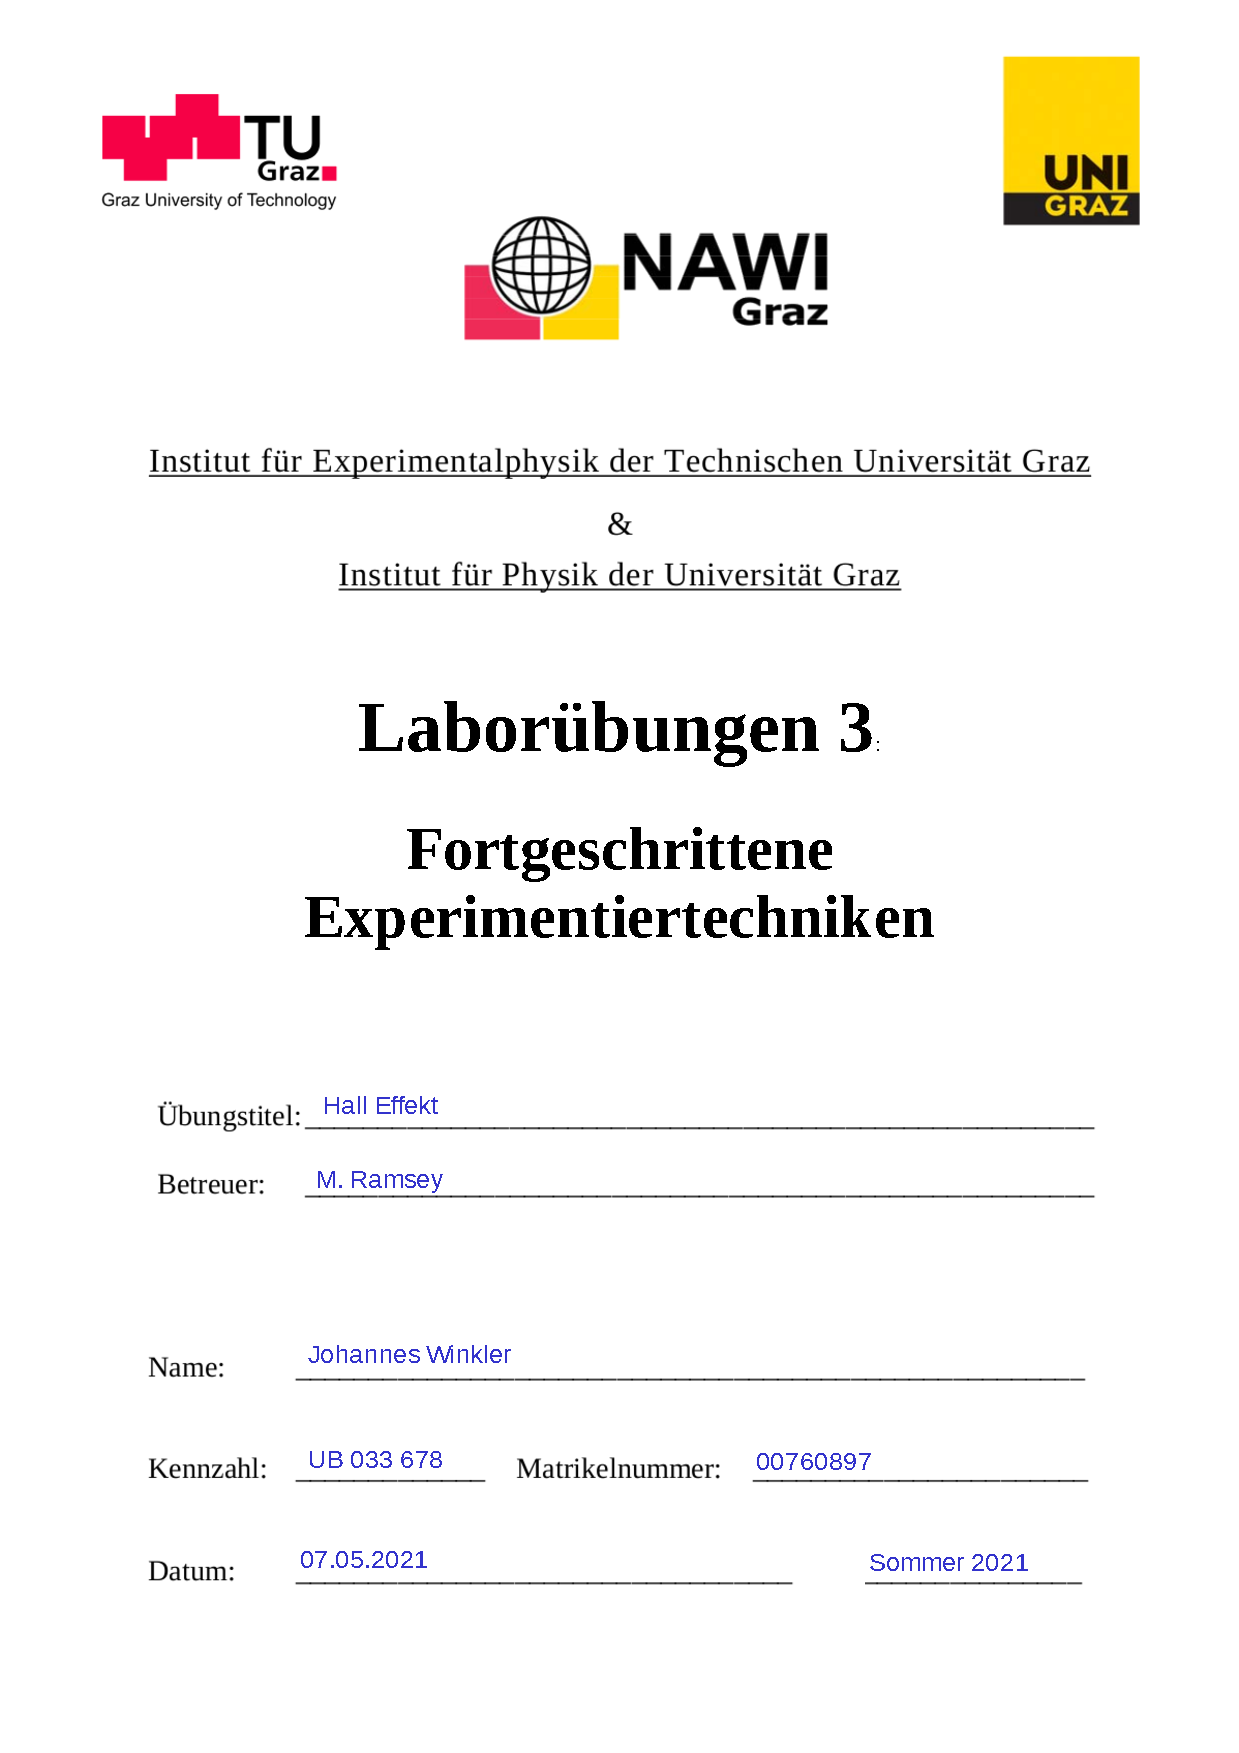
\includepdf{Deckblatt_neu_custom.pdf}

\tableofcontents
\newpage

\pagestyle{fancy}

\section{Aufgabenstellung}

Es ist die Hall-Konstante und die Ladungsträgerkonzentration eines Ge-Kristalls zu bestimmen. Dies sollte durch mehrfache Messungen der Hallspannung bei gegebenem Querstrom und Magnetfeldstärke bestimmt werden.


%\begin{figure}[H]
%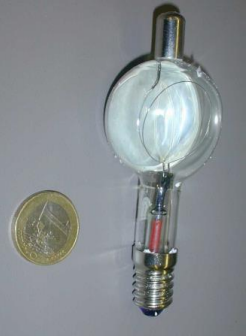
\includegraphics[scale=1.4]{versuch3.png}
%\caption{Vakuum Photozelle. Quelle: \cite{moodle}}
%\end{figure}

\section{Grundlagen}


\begin{figure}[H]
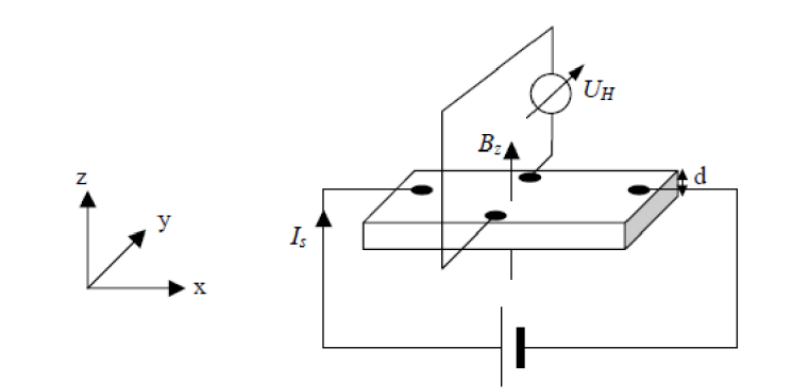
\includegraphics[scale=1.4]{versuch2.png}
\caption{Grundlagen des Hall Effekts. Quelle: \cite{moodle}}
\label{fig:grundlagen}
\end{figure}

Grafik~\ref{fig:grundlagen} zeigt das Prinzip des Hall Effekts. Durch einen Kristall (in der Skizze quaderförmig) fließt ein Querstrom $I$ in x-Richtung. Zusätzlich wird in z-Richtung ein Magnetfeld angelegt. Die durch $I$ bewegten Ladungsträger fließen nun mit einer bestimmten Geschwindigkeit $v$ (Driftgeschwindigkeit) durch das Magnetfeld. Dabei werden sie von der Lorentzkraft
\begin{align*}
F = q\cdot (\vec{v} \times \vec{B})
\end{align*}
abgelenkt, wobei aufgrund der Orthogonalität auch mit den skalaren Größen gerechnet werden kann. Also gilt für die Lorentzkraft
\begin{align*}
F = q\cdot v\cdot B
\end{align*}
wobei $q \in\{e,-e\}$ betragsmäßig die Elementarladung ist und je nach Dotierung ein positives oder negatives Vorzeichen hat. Durch die Lorentzkraft werden positive und negative Ladungen in entgegen gesetzte Richtung abgelenkt, sodass sich in y-Richtung ein elektrisches Feld $E_H$ bildet. Dieses wird solange vergrößert, bis die Coulombkraft die Lorentzkraft kompensiert und ein Gleichgewichtszustand eintritt. Dann gilt
\begin{align*}
q\cdot E_H = q\cdot v \cdot B
\end{align*}
Division durch $q$ und Einsetzen der Driftgeschwindigkeit ergibt sich
\begin{align*}
E_H = \frac{I}{\nu\cdot A\cdot q} \cdot B
\end{align*}
wobei $A$ als (entgegen Grafik~\ref{fig:grundlagen}) quadratische Querschnittsfläche mit $A=d^2$ angenommen wird und $\nu \in \{n,p\}$ die Ladungsträgerdichte ist (je nach Dotierung). Da $d$ hinreichend klein ist, wird das elektrische Feld innerhalb des Kristalls als konstant angenommen, sodass $U_H = E_H\cdot d$ gilt. Es folgt
\begin{align*}
U_H = \frac{I\cdot B}{\nu \cdot q \cdot d}
\end{align*}
oder anders geschrieben
\begin{align}
U_H = R_H \cdot \frac{I\cdot B}{d}
\label{eq:hall}
\end{align}
wobei für die Hall-Konstante $R_H = \dfrac{1}{\nu\cdot q}$ gilt
\begin{align*}
R_H = \begin{cases} -\dfrac{1}{n\cdot e} & \text{für Elektronenleitung} \\ 
& \\
 +\dfrac{1}{p\cdot e} & \text{für Löchterleitung} \end{cases}
\end{align*}



\section{Versuchsaufbau}

\begin{figure}[H]
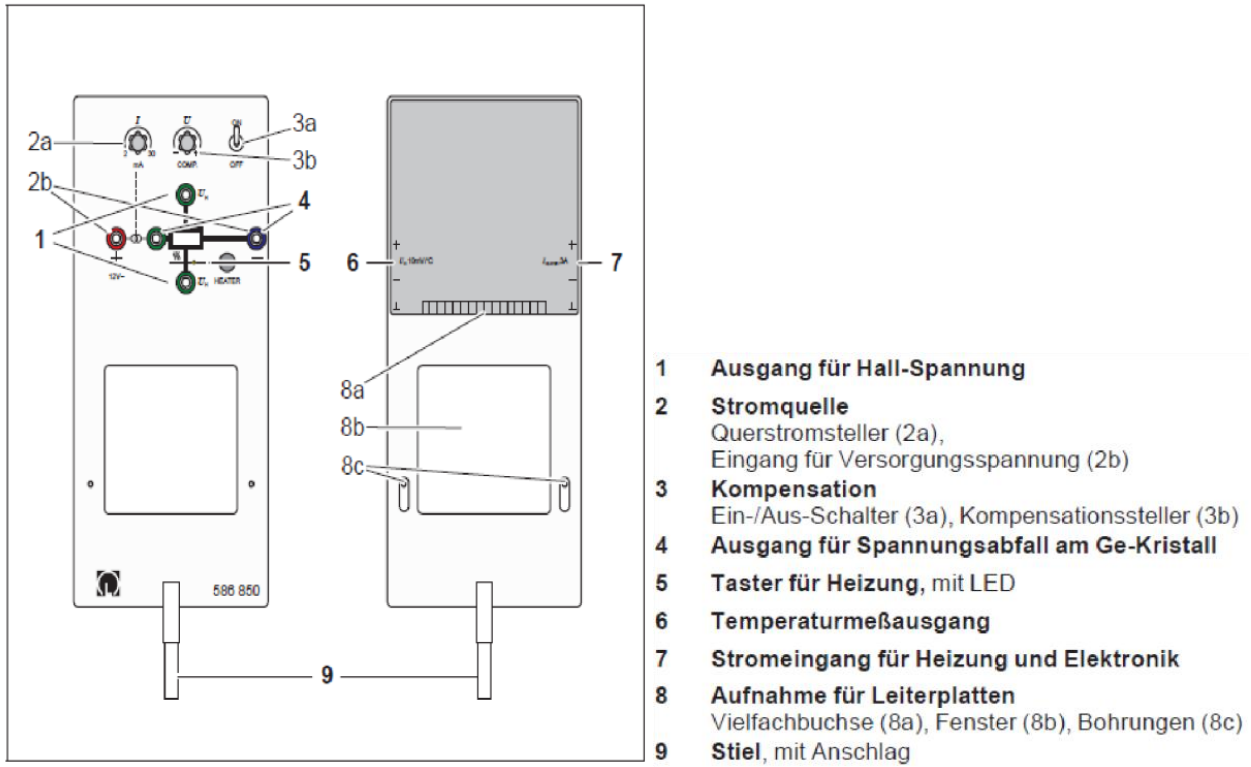
\includegraphics[scale=1.4]{versuch1.png}
\caption{Aufbau des Versuchs. Quelle: \cite{moodle}}
\end{figure}



\section{Geräteliste}


\begin{table}[H]
\caption{Liste der verwendeten Geräte}
~
\begin{tabular}{l|l}
 & Geräte  \\
\hline
1 & Versuchsapparatur für Hall-Effekt mit Ge-Kristall mit $d=(1.0\pm0.1)~$mm\\
2 & Elektromagnet \\
3 & Netzgerät für Elektromagneten \\
4 & Computer mit Cassy-Lab 2 \\
5 & Cassy Sensor
\end{tabular}

\end{table}

\newpage

\section{Durchführung und Messergebnisse}

Für die Messung wurde die magnetische Flussdichte zwischen $B=-250~$mT und $B=250~$mT in Schritten von $50~$mT variiert. Der Strom durch den Kristall wird beginnend bei $I=2~$mA in $5~$mA Schritten auf bis zu $32~$mA erhöht. Insgesamt ergeben sich die Messwerte

\begin{table}[H]
\caption{Messwerte für die Hall-Spannung $U_B$ in mV bei gegebenen Magnetfeld $B$ in mT und gegebenen Querstrom $I$ in mA.}
\begin{tabular}{c|ccccccccccc}
I & $U_{-250}$ & $U_{-200}$ & $U_{-150}$ & $U_{-100}$ & $U_{-50}$ & $U_{0}$ & $U_{50}$ & $U_{100}$ & $U_{150}$ & $U_{200}$ & $U_{250}$\\
\hline2  & -2.3 & -1.6 & -1.1 & -0.5 & 0.1 & 0.8 & 1.4 & 1.9 & 2.6 & 3.2 & 3.8\\ 
7  & -7.6 & -5.8 & -3.8 & -2.0 & 0.0 & 1.8 & 3.7 & 5.5 & 7.4 & 9.3 & 11.2\\ 
12  & -13.4 & -10.2 & -6.9 & -3.6 & -0.3 & 3.0 & 6.2 & 9.4 & 12.8 & 16.0 & 19.2\\ 
17  & -19.2 & -14.6 & -9.9 & -5.2 & -0.6 & 3.0 & 8.7 & 13.3 & 18.1 & 22.7 & 27.3\\ 
22  & -25.4 & -19.3 & -13.2 & -7.0 & -1.0 & 5.2 & 11.3 & 17.6 & 23.7 & 29.8 & 35.8\\ 
27  & -30.6 & -23.5 & -16.0 & -8.6 & -1.3 & 6.2 & 13.7 & 21.1 & 28.5 & 35.9 & 43.2\\ 
32  & -36.0 & -27.5 & -18.9 & -10.1 & -1.6 & 7.2 & 16.0 & 24.6 & 33.3 & 42.0 & 50.6\\ 

\end{tabular}
\label{tab:messung}
\end{table}

Die Messwerte werden nun in Grafik~\ref{fig:messung1} dargestellt, wobei die Hallspannung abhängig vom Querstrom angegeben wird.
\begin{figure}[H]
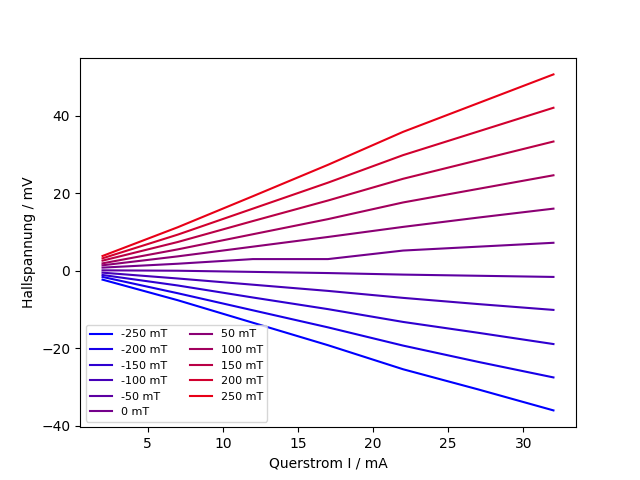
\includegraphics[scale=0.7]{regression_I.png}
\caption{Grafische Darstellung der Hall-Spannung aus Tabelle~\ref{tab:messung} in Abhängigkeit zum Querstrom.}
\label{fig:messung1}
\end{figure}



Die Messwerte werden nun in Grafik~\ref{fig:messung2} dargestellt, wobei die Hallspannung abhängig von der magnetischen Flussdichte angegeben wird.
\begin{figure}[H]
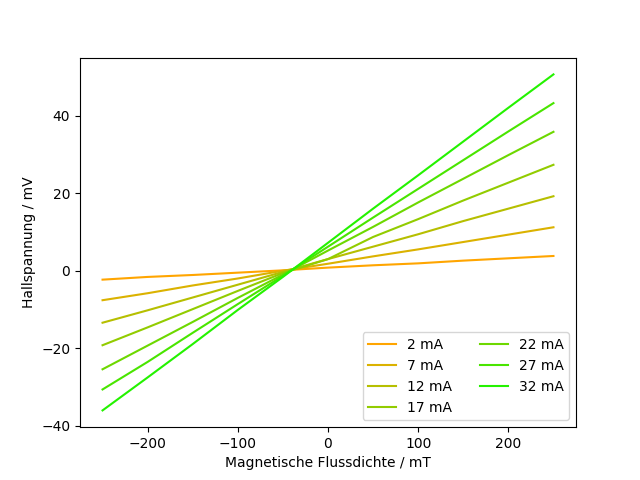
\includegraphics[scale=0.7]{regression_B.png}
\caption{Grafische Darstellung der Hall-Spannung aus Tabelle~\ref{tab:messung} in Abhängigkeit zur magnetischen Flussdichte.}
\label{fig:messung2}
\end{figure}


\section{Auswertung}

Nach Gleichung~\eqref{eq:hall} gilt folgende Beziehung
\begin{align}
U_H = R_H \cdot \frac{I\cdot B}{d}
\end{align}
Wobei diese auch auf die Arten
\begin{align}
U_H &= \frac{R_H\cdot B}{d} \cdot I \label{eq:regrI} \\
U_H &= \frac{R_H\cdot I}{d} \cdot B \label{eq:regrB}
\end{align}
geschrieben werden kann. Man kann daher die Hall-Konstante sowohl durch Regression zwischen $I$ und $U_H$, als auch bei einer Regression zwischen $B$ und $U_H$ berechnen.

Es empfiehlt sich praktischerweise, die Hall-Konstante durch eine Regression zwischen $B$ und $U_H$ zu bestimmen, wobei $I$ konstant gehalten wird. Das liegt zum einen an der Messreihe für $B=0$. Da hätte man zur Berechnung von $R_H = \dfrac{k\cdot d}{B}$ eine Nulldivision. Das Problem stellt sich für die Regression zwischen $B$ und $U_H$ nicht, da $I\neq0$ gilt. Die Ergebnisse sind in Tabelle~\ref{tab:auswertung_B_U} zu sehen.

\begin{table}[H]
\caption{Berechnung der Regressionsgeraden~\eqref{eq:regrB} zwischen $B$ und $U_H$ bei fixem Strom $I$. Aus der Steigung $k$ wird die Hall-Konstante $R_H = k\cdot d/I$ berechnet und daraus wiederum die Ladungsträgerkonzentration $p=(R_H\cdot e)^{-1}$.}
\begin{tabular}{r|r|r|r}
$I$ / mA & $k$ / mV/T & $R_H$ / m$^3$/C & p / m$^{-3}$ \\
\hline
2 & 12 & 6.08 $\cdot 10^{-3}$ & 103$\cdot 10^{19}$ \\7 & 38 & 5.37 $\cdot 10^{-3}$ & 116$\cdot 10^{19}$ \\12 & 65 & 5.45 $\cdot 10^{-3}$ & 115$\cdot 10^{19}$ \\17 & 93 & 5.48 $\cdot 10^{-3}$ & 114$\cdot 10^{19}$ \\22 & 123 & 5.58 $\cdot 10^{-3}$ & 112$\cdot 10^{19}$ \\27 & 148 & 5.48 $\cdot 10^{-3}$ & 114$\cdot 10^{19}$ \\32 & 174 & 5.42 $\cdot 10^{-3}$ & 115$\cdot 10^{19}$ \\
\end{tabular}
\label{tab:auswertung_B_U}
\end{table}

Wenn man in Tabelle~\ref{tab:auswertung_B_U} die Zeile für $I=2~$mA als Ausreisser sieht, dann gilt offenbar für die Hall-Konstante durch Bildung von Mittelwert und Standardabweichung
\begin{align*}
R_H &= (5.46 \pm 0.06)\cdot 10^{-3} ~\text{m}^3/\text{C} \\
p &= (114\pm1) \cdot 10^{19} ~\text{m}^{-3}
\end{align*}



\section{Diskussion}

Durch die positive Hall-Konstante zeigt sich, dass es sich um Lochleitung handelt und daher die Ladungsträgerdichte als $p$ geschrieben wird. Der Zahlenwert selbst ist für Germanium schwer aufzutreiben. Außerdem hängt dieser noch von verschiedenen Faktoren ab, zB. von Reinheit und Temperatur und Dotierung.




\section{Zusammenfassung}

In diesem Experiment war die Hall-Konstante und die Ladungsträgerdichte eines Germanium-Kristalls zu bestimmen. Es wurden die folgenden Werte bestimmt.
\begin{align*}
R_H &= (5.46 \pm 0.06)\cdot 10^{-3} ~\text{m}^3/\text{C} \\
p &= (114\pm1) \cdot 10^{19} ~\text{m}^{-3}
\end{align*}



\begin{thebibliography}{9}
\bibitem{moodle} G. Koller: Skript zum Hall Effekt aus dem Moodle der Karl-Franzens Universität, Institut für Physik, 07.05.2021.
\bibitem{messmethoden}  R. Dämon: Einführung in die physikalischen Messmethoden, Graz 2016.
\bibitem{demtroeder} W. Demtröder: \emph{Experimentalphysik 2 - Elektrizität  und Optik}, 7. Auflage, 2017.
\bibitem{python} Python-Skript zur Berechnung der Daten, zur Visualisierung und zum Generieren von \LaTeX-Code für diesen Bericht.
\end{thebibliography}


\newpage 
%\appendix
%\section{Python Skript}



\definecolor{commentgreen}{RGB}{2,112,10}
\definecolor{eminence}{RGB}{108,48,130}
\definecolor{weborange}{RGB}{255,165,0}
\definecolor{frenchplum}{RGB}{129,20,83}

\lstdefinelanguage{python}{
    morekeywords={def, for, range, abs, return},
    otherkeywords={<-,->, |>, \%\{, \}, \{, \, (, )},
    sensitive=true,
    morecomment=[l]{\#},
    morecomment=[n]{/*}{*/},
    morecomment=[s][\color{purple}]{:}{\ },
    morestring=[s][\color{orange}]"",
    commentstyle=\color{commentgreen},
    keywordstyle=\color{eminence},
    stringstyle=\color{red},
	basicstyle=\ttfamily,
	breaklines,
	showstringspaces=false,
	frame=tb
}
%\lstinputlisting[language=Python,captionpos=b, label=lst:test,caption={Auswertung}]{script.py}

%\lstinputlisting[language=Python,captionpos=b, label=lst:test,caption={Bessel Auswertung}]{generate_numbers_bessel.py}



\end{document}